\documentclass[11pt]{jarticle}

\usepackage[dvipdfmx]{graphicx}
\usepackage{listings}
\usepackage{url}

\lstset{
    basicstyle={\ttfamily\small}, %書体の指定
    frame=tRBl, %フレームの指定
    framesep=10pt, %フレームと中身(コード)の間隔
    breaklines=true, %行が長くなった場合の改行
    linewidth=16cm, %フレームの横幅
    lineskip=-0.5ex, %行間の調整
    tabsize=2 %Tabを何文字幅にするかの指定
}

\setlength{\oddsidemargin}{-6.35mm}
\setlength{\textwidth}{171.9mm}

\begin{document}

\title{画像処理実験 第7回}
\author{09430565\\大橋虎ノ介}
\date{\number\year 年\number\month 月\number\day 日}
\maketitle

\section{概要}

 今回の実験では,貪欲法により得られた特徴点の組の中から
正しい特徴点の組を4つ選ぶ処理を記述する.

ここではRANSACと呼ばれるアルゴリズムを用いて特徴点の自動対応付けを行う.

\section{正しさの指標}

ここでは,4つの特徴点の組を無作為に抽出し,正しさを計算する.
この試行を多数回行い,最も正しい組み合わせを探し出す.

正しさの指標は,次のように決定する.

まず,無作為に選び出した4つの特徴点を対応付ける射影変換行列を
最小二乗法によって求める.
もし,選び出した4つの特徴点の組が正しければ,この射影変換行列を用いて
ほかの特徴点も対となる特徴点へ射影変換可能である.
なので,射影変換可能である特徴点の組の数を正しさの指標とする.

\section{RANSACの実装}

以下のようにRANSAC関数を実装した.

RANSAC関数は,最も正しさの指標が高かった時の
射影変換行列を格納するBestH配列と
特徴点の組の座標wを引数として受け取る.

initRndAry関数とchooseFourNumbers関数は
rndAry配列の内容をシャッフルする.
特徴点の組の座標wの添え字としてrndAryを指定することで,
無作為に抽出するという動作を実装している.

calcHomography関数は最小二乗法によって射影変換行列を求める.
calcScore関数はcalcHomography関数によって求めた射影変換行列
の正しさを計算する.

上の試行を定数TRIALによって定められた回数繰り返し,
最も正しいとされた射影変換行列bestH[3][3]に格納する.

\begin{lstlisting}
void ransac(double bestH[3][3], double w[][4]) {
    int best_score = 0;
    int rndAry[MAX];
    int score;
    Matrix* cmA, * vt, * mtR, * tmp;
    cmA = MatrixAlloc(8, 8);
    vt = MatrixAlloc(1, 8);
    mtR = MatrixAlloc(8, 8);
    tmp = MatrixAlloc(1, 8);
    initRndAry(rndAry);
    for (int trial = 0; trial < TRIAL; trial++) {
        double H[3][3];
        chooseFourNumbers(rndAry);
        calcHomography(H, w, rndAry, cmA, vt, mtR, tmp);
        score = calcScore(H, w);
        if (best_score < score) {
            printf("score: %d\n", score);
            for (int i = 0; i < 3; i++) for (int j = 0; j < 3; j++) {
                bestH[i][j] = H[i][j];
            }
            best_score = score;
        }
    }

}
\end{lstlisting}

\begin{lstlisting}
void calcHomography(double H[3][3], double w[][4], int rndAry[MAX], Matrix* cmA, Matrix* vt, Matrix* mtR, Matrix* tmp) {
    for (int i = 0; i < 4; i++) {
        Elem(cmA, 0, i * 2) = w[rndAry[i]][0];
        Elem(cmA, 1, i * 2) = w[rndAry[i]][1];
        Elem(cmA, 2, i * 2) = 1;
        Elem(cmA, 3, i * 2) = 0;
        Elem(cmA, 4, i * 2) = 0;
        Elem(cmA, 5, i * 2) = 0;
        Elem(cmA, 6, i * 2) = -w[rndAry[i]][0] * w[rndAry[i]][2];
        Elem(cmA, 7, i * 2) = -w[rndAry[i]][1] * w[rndAry[i]][2];
        Elem(cmA, 0, i * 2 + 1) = 0;
        Elem(cmA, 1, i * 2 + 1) = 0;
        Elem(cmA, 2, i * 2 + 1) = 0;
        Elem(cmA, 3, i * 2 + 1) = w[rndAry[i]][0];
        Elem(cmA, 4, i * 2 + 1) = w[rndAry[i]][1];
        Elem(cmA, 5, i * 2 + 1) = 1;
        Elem(cmA, 6, i * 2 + 1) = -w[rndAry[i]][0] * w[rndAry[i]][3];
        Elem(cmA, 7, i * 2 + 1) = -w[rndAry[i]][1] * w[rndAry[i]][3];
        Elem(vt, 0, i * 2) = w[rndAry[i]][2];
        Elem(vt, 0, i * 2 + 1) = w[rndAry[i]][3];
    }
    MatrixQRDecompColMajor(mtR, cmA);
    MatrixMultT(tmp, vt, cmA);
    MatrixSimeqLr(tmp, mtR);
    for (int i = 0; i < 3; i++) for (int j = 0; j < 3; j++) {
        if (i == 2 && j == 2) {
            H[i][j] = 1;
        }
        else {
            H[i][j] = tmp->data[i * 3 + j];
        }
    }
}
\end{lstlisting}

\begin{lstlisting}
 int calcScore(double H[3][3], double w[][4]) {
    int score = 0;
    for (int i = 0; i < 30; i++) {
        double x = w[i][0], y = w[i][1],
            u = w[i][2], v = w[i][3],
            x_prime, y_prime, z_prime, // 変換行列と (x,y,1)^T の積
            du, dv; // (x,y) を変換した座標(第2回の概要を参照)と (u,v) の差.
        
        x_prime = H[0][0] * w[i][0] + H[0][1] * w[i][1] + H[0][2];
        y_prime = H[1][0] * w[i][0] + H[1][1] * w[i][1] + H[1][2];
        z_prime = H[2][0] * w[i][0] + H[2][1] * w[i][1] + H[2][2];
        
        du = x_prime / z_prime - u;
        dv = y_prime / z_prime - v;
        if (du * du + dv * dv < 10) score++;

    }
    return score;
}
\end{lstlisting}

\section{実装結果}

以下の2つの画像(0.jpg, 1.jpg)と,便宜的に用意した特徴点を入力した.

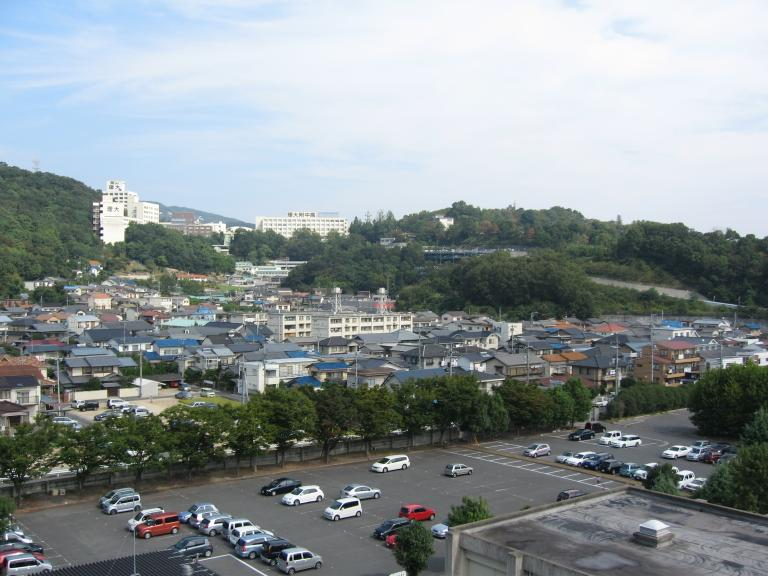
\includegraphics[scale=.3]{./img/0.jpg}
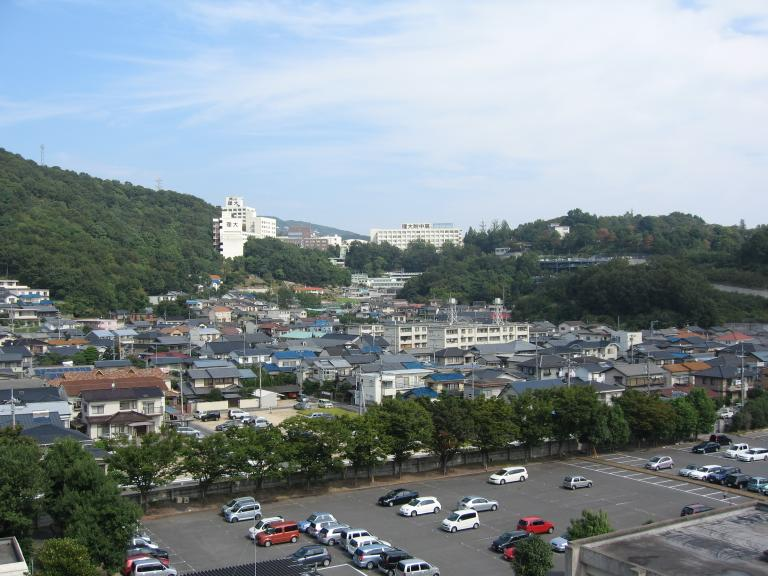
\includegraphics[scale=.3]{./img/1.jpg}

\begin{lstlisting}
    int x1[][2] = { \\0.jpgの特徴点
        234, 529,
        237, 530,
        294, 560,
        336, 512,
        685, 481,
        355, 506,
        296, 496,
        615, 439,
        384, 464,
        293, 497,
        353, 497,
        113, 398,
        317, 494,
        403, 462,
        195, 519,
        202, 520,
        99, 210,
        116, 407,
        96, 229,
        108, 199,
    }, N1 = 20;
    int x2[][2] = {\\1.jpgの特徴点
        354, 539,
        352, 537,
        452, 524,
        473, 518,
        413, 507,
        410, 508,
        471, 511,
        234, 409,
        743, 453,
        434, 505,
        500, 476,
        314, 528,
        42, 295,
        521, 473,
        320, 529,
        219, 226,
        237, 417,
        261, 522,
        333, 536,
        216, 247,
    }, N2 = 20;
\end{lstlisting}

次のような画像が出力された.

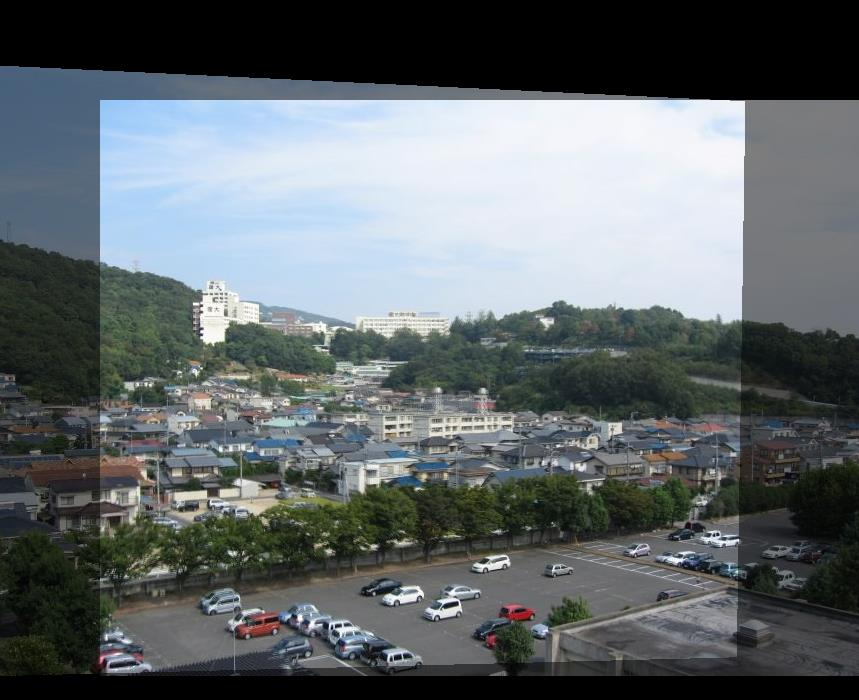
\includegraphics[scale=.5]{./img/out.jpg}

\section{考察}

今回の実験では,貪欲法により得られた特徴点の組の中から
RANSACというアルゴリズムを用いて,
正しい特徴点の組を4つ選ぶ処理を記述した.

N組の特徴点の組の中から4つ選び出すやり方は次のとおりである.
\[{}_n C_4 = \frac{n!}{4!(n-4)!}\\
    = \frac{n(n-1)(n-2)(n-3)}{24}\\
    \sim n^{4}/24\]

計算量はO($n^{4}$)であるので,画像サイズが大きくなると
特徴点の数が多くなり,計算に時間がかかる.
RANSACを用いることで,最適でないにしても正解に近い
答えを短い時間で出すことができた.

\end{document}